\documentclass[../../course]{subfiles}

\renewcommand\thesection{\arabic{section}}


\begin{document}

\def\freqXOne{28}
\def\freqXTwo{56}
\def\freqXThree{56.1}

\def\sampFreqMuchLess{\textbf{(a):} $f_{s} = \frac{4 \times 28}{2} = 56 \si{Hz}$}
\def\sampFreqNorm{\textbf{(b):} $f_{s} = 4 \times 28 = 112 \si{Hz}$}
\def\sampFreqSligGreat{\textbf{(c):} $f_{s} = (4 \times 28) + 10 = 122 \si{Hz}$}
\def\sampFreqMuchGreat{\textbf{(d):} $f_{s} = 4 \times 28 \times 6 = 672 \si{Hz}$}

\section{Taking DTFT of the Complex Sequences} \label{sec:wrkTakingDTFTCplxSeqs}

In the previous section, we generated a bunch of \emph{complex sequences}. And
picked $4$ sequences for further analysis. In this section we will be taking
\textsc{dtft} of those sequences. But before that, we need to take a look at what
a \textsc{dtft} is and how to compute them using \textsc{python}.

\subsection{Discrete Time Fourier Transform}

Discrete Time Fourier Transform, aka, \textsc{dtft} transforms \emph{discrete time}
samples into a \emph{continuous} signal in the \emph{frequency} domain. \textsc{dtft}
is basically a special case of another transform known as $\mathcal{Z}$\textsc{-transform}.
$\mathcal{Z}$\textsc{-transform} can be mathematically described as,

\begin{align}
    X(z) = {\mathcal{Z}}\{x[n]\} = \sum_{n = - \infty}^{\infty} x[n] z^{-n}
\end{align}

where,

\begin{itemize} [label=]

    \item ${\mathcal{Z}}\{x[n]\}$: is the $\mathcal{Z}$\textsc{-transform}.
    \item $x[n]$: is the input sequence, which was sampled with a
        particular \emph{sampling frequency}, $f_{s}$.
    \item $z$: is a \emph{complex number}, in the form $A e^{-j \omega}$.

        where,

        \begin{itemize} [label=]
            \item $A$: is the \emph{real part} or the \emph{amplitude}.
            \item $\omega$: is the \emph{complex argument} in radians.
        \end{itemize}

\end{itemize}

\textsc{dtft} is a special case of $\mathcal{Z}$\textsc{-transform}, where we take $A$
as $1$. Mathematically, we can describe \textsc{dtft} as,

\begin{align}
    X(e^{j \omega}) &= X(z) |_{z = e^{j \omega}} \\
    &= \sum_{n = - \infty}^{\infty} x[n] z^{-n} \Big|_{z = e^{jw}} \\
    &= \sum_{n = - \infty}^{\infty} x[n] e^{-j w n} \label{eqn:dtftOmega}
\end{align}

Where $\omega$ can be substituted with $2 \pi f$, then the \textsc{dtft} becomes,

\begin{align}
    X(e^{j 2 \pi f}) &= \sum_{n = - \infty}^{\infty} x[n] e^{-j 2 \pi f n}
    \label{eqn:dtftFreq}
\end{align}

Now eq. (\ref{eqn:dtftOmega}) becomes a function of \emph{frequency} $f$
instead of \emph{angular frequency} $\omega$. One thing to \textsc{note} is that,
\emph{sweeping} $f$ in eq. (\ref{eqn:dtftFreq}) from $0$ to $1$ will result in same
output as \emph{sweeping} $\omega$ in eq. (\ref{eqn:dtftOmega}) from $0$ to $2 \pi$.
Another interesting thing about this \emph{transform} is that the $e^{-j 2 \pi f n}$ will
\emph{scales} and \emph{wraps} the \emph{frequencies} from $0$ to $\infty$ around
the \textsc{Unit Circle} in the $\mathcal{Z} \textsc{-plane}$. This will become
important as we compute the \textsc{dtft}s. The Figure \ref{fig:wrapFreqUnitCircle}
attempts to visualizes this interesting concept.

\begin{figure}
    \centering
    \adjustbox{max width = 1\textwidth} {
        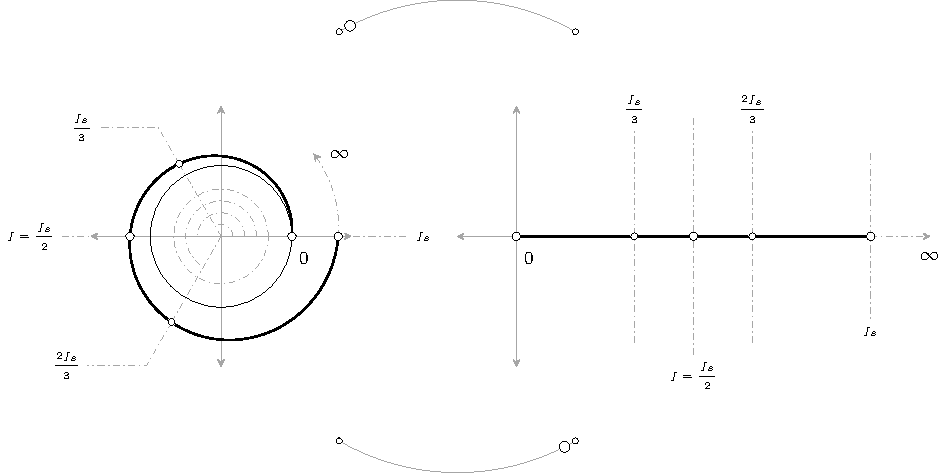
\includegraphics[height = 1\textheight] {tikzpics/epicWrapFreqUnitCircle.pdf}
    }
    \captionof{figure} {
        Wrapping frequencies around the \textsc{Unit Circle} in $\mathcal{Z}\textsc{-plane}$
    }
    \label{fig:wrapFreqUnitCircle}
\end{figure}

\subsection{Implementing DTFT using Python}

We essentially need to take \textsc{dtft} of several\footnote{actually $4$, still
more than $1$.} sequences. So it will be handy to implement a \emph{factory}, that
will take a \emph{sequence} and returns a \emph{dtft function} that can be called
with different \emph{frequencies} and returns it's corresponding value. Let us call
this \emph{function} the \mintinline{python}{dtft_factory}.

%python/dtft_factory.py%
\begin{minted}[breaklines, autogobble, mathescape] {python}
    import numpy as np

    def dtft_factory(cplx_seq):

        def dtft(freq):
            sum = 0
            # see eq. ($\ref{eqn:dtftFreq}$)
            for n, cplx in enumerate(cplx_seq):
                sum = sum + cplx * np.exp(-1j * 2 * np.pi * freq * n)
            return sum

        return dtft
\end{minted}

Now, let's implement another \emph{function} that will returns another
\emph{function}\footnote{yes, of course.} that can be called with $n = 0, 1, 2, ...$
to generate the \emph{sequence} with specified \emph{sampling frequency}, \emph{real}
and \emph{imaginary} parts. Let's call this \emph{function} \mintinline{python}{cplx_factory}

%python/cplx_factory.py%
\begin{minted}[breaklines, autogobble, mathescape] {python}
    import numpy as np

    def cplx_factory(samp_freq, real_freq, imag_freq):
        samp_period = 1 / samp_freq
        return lambda n: np.sin(
            2 * np.pi * real_freq * (n * samp_period)
        ) + 1j * np.sin(
            2 * np.pi * imag_freq * (n * samp_period)
        )
\end{minted}

Let's implement yet another \emph{function} that will make our life easier by
\emph{mixing} and \emph{generating} the \textsc{dtft} for two given \emph{frequencies}\footnote{one
as \emph{real} and one as \emph{imaginary}.}. As depicted in Figure \ref{fig:wrapFreqUnitCircle}
we only need to evaluate the \textsc{dtft} from $0$ to $1$ range\footnote{in the case
of eq. (\ref{eqn:dtftFreq}).} and need to \emph{rescale} it back.

%python/gen_dtft_seq.py%
\begin{minted}[breaklines, autogobble, mathescape] {python}
    def gen_dtft_seq(
        samp_count, samp_freq, real_freq, imag_freq, dtft_samp_count
        ):

        cplx_fn = cplx_factory(
            samp_freq = samp_freq,
            real_freq = real_freq,
            imag_freq = imag_freq
        )

        cplx_seq = np.ndarray(samp_count, dtype = np.cdouble)

        for i in range(samp_count):
            cplx_seq[i] = cplx_fn(i)

        freq = np.linspace(0, 1, dtft_samp_count)

        dtft_fn = dtft_factory(cplx_seq = cplx_seq)
        dtft_seq = dtft_fn(freq)

        # scaling back the freq from ($0$ - $1$) to ($0$ - $f_{s}$)
        return freq * samp_freq, dtft_seq, cplx_seq
\end{minted}

Now we could just call \mintinline{python}{gen_dtft_seq} with appropriate \emph{arguments}
and it will return the \mintinline{python}{dtft_seq} and its corresponding \emph{frequencies}.
Let's take a bunch of \textsc{dtft}s with different \emph{sampling frequencies}.

%python/taking_dtft.py%
\begin{minted}[breaklines, autogobble, mathescape] {python}
    import pandas as pd

    X = 28

    cplx_seqs = [
        {
            "name": "complex_a",
            "real_freq": X,
            "imag_freq": X,
            # we will fill this later, for taking 64 point DTFT
            "sequences": {},
        },
        {
            "name": "complex_b",
            "real_freq": X,
            "imag_freq": 2 * X,
            "sequences": {},
        },
        {
            "name": "complex_c",
            "real_freq": X,
            "imag_freq": (2 * X) + 0.1,
            "sequences": {},
        },
        {
            "name": "complex_f",
            "real_freq": 2 * X,
            "imag_freq": (2 * X) + 0.1,
            "sequences": {},
        },
    ]

    samp_freqs = {
        "normal":           int(4 * X),
        "slightly_greater": int(4 * X + 10),
        "much_greater":     int(4 * X * 6),
        "much_lesser":      int(4 * X / 2),
    }

    samp_count = 32

    dtft_samp_count = 2000

    for cplx in cplx_seqs:

        for samp_freq in samp_freqs:

            freq, dtft_seq, cplx_seq = gen_dtft_seq(
                samp_count = samp_count,
                samp_freq = samp_freqs[samp_freq],
                real_freq = cplx["real_freq"],
                imag_freq = cplx["imag_freq"],
                dtft_samp_count = dtft_samp_count
            )

            # keeping generated sequences for taking 64 point DTFT
            cplx["sequences"][samp_freq] = cplx_seq

            data = pd.DataFrame(
                data = {
                    "real": dtft_seq.real,
                    "imag": dtft_seq.imag,
                },
                index = freq
            )

            data.to_csv(
                "../data/dtft_" + cplx["name"] + "_" + samp_freq + "_32.csv",
                sep = " ", index_label = "freq"
            )
\end{minted}

We have generated \textsc{dtft}s for our \emph{sequences} with
different \emph{sampling frequencies}, and \mintinline{python} {cplx_seqs}
dictionary has all those generated \emph{input sequences}. Now we need
to pad them with $32$ zeros and find the \textsc{dtft}s of those sequences.
Let's quickly implement another \emph{function} for that. Let it be
\mintinline{python}{gen_dtft_seq_64}.

%python/gen_dtft_seq_64.py%
\begin{minted}[breaklines, autogobble, mathescape] {python}
    def gen_dtft_seq_64(
        cplx_seq, samp_freq, dtft_samp_count
        ):

        cplx_seq = np.concatenate(
            [cplx_seq, np.zeros(32, dtype = np.cdouble)]
        )

        freq = np.linspace(0, 1, dtft_samp_count)

        dtft_fn = dtft_factory(cplx_seq = cplx_seq)
        dtft_seq = dtft_fn(freq)

        # scaling back the freq from ($0$ - $1$) to ($0$ - $f_{s}$)
        return freq * samp_freq, dtft_seq, cplx_seq
\end{minted}

Now let's take the \textsc{dtft}s of those sequences using this
\mintinline{python}{gen_dtft_seq_64}.

%python/taking_dtft_64.py%
\begin{minted}[breaklines, autogobble, mathescape] {python}
    dtft_samp_count = 2000

    for cplx in cplx_seqs:
        for seq_name in cplx["sequences"]:
            freq, dtft_seq, _ = gen_dtft_seq_64(
                cplx_seq = cplx["sequences"][seq_name],
                samp_freq = samp_freqs[seq_name],
                dtft_samp_count = dtft_samp_count
            )

            data = pd.DataFrame(
                data = {
                    "real": dtft_seq.real,
                    "imag": dtft_seq.imag,
                },
                index = freq
            )

            data.to_csv(
                "../data/dtft_" + cplx["name"] + "_" + seq_name + "_64.csv",
                sep = " ", index_label = "freq"
            )
\end{minted}

\pagebreak

\subsection{DTFT of Complex A} \label{ssec:dtftCplxA}

\begin{itemize} [label=]

    \item \textbf{Sequence:} $\sin(2 \pi \freqXOne t) + j \sin(2 \pi \freqXOne t)$

\end{itemize}

\subsubsection{DTFT with 32 Samples}

\begin{itemize} [label=]

    \item \sampFreqMuchLess
        \begin{itemize} [label=]
            \item To much \emph{aliasing}, can barely distinguish $\freqXOne \si{Hz}$.
        \end{itemize}

    \item \sampFreqNorm
        \begin{itemize} [label=]
            \item \emph{Real} and \emph{imaginary} parts have same frequency, therefore that \emph{bulge}
                at the pulse near $\freqXOne$.
        \end{itemize}

    \item \sampFreqSligGreat
        \begin{itemize} [label=]
            \item Similar to (b).
        \end{itemize}

    \item \sampFreqMuchGreat
        \begin{itemize} [label=]
            \item Similar to (b) and (c).
        \end{itemize}

    \item \textbf{Inference:} We can distinguish almost two of the \emph{frequencies} from four
        of the different \emph{sampling frequencies}.

\end{itemize}

\vfill

\begin{figure} [H]
    \centering
    \adjustbox{max width = 1\textwidth} {
        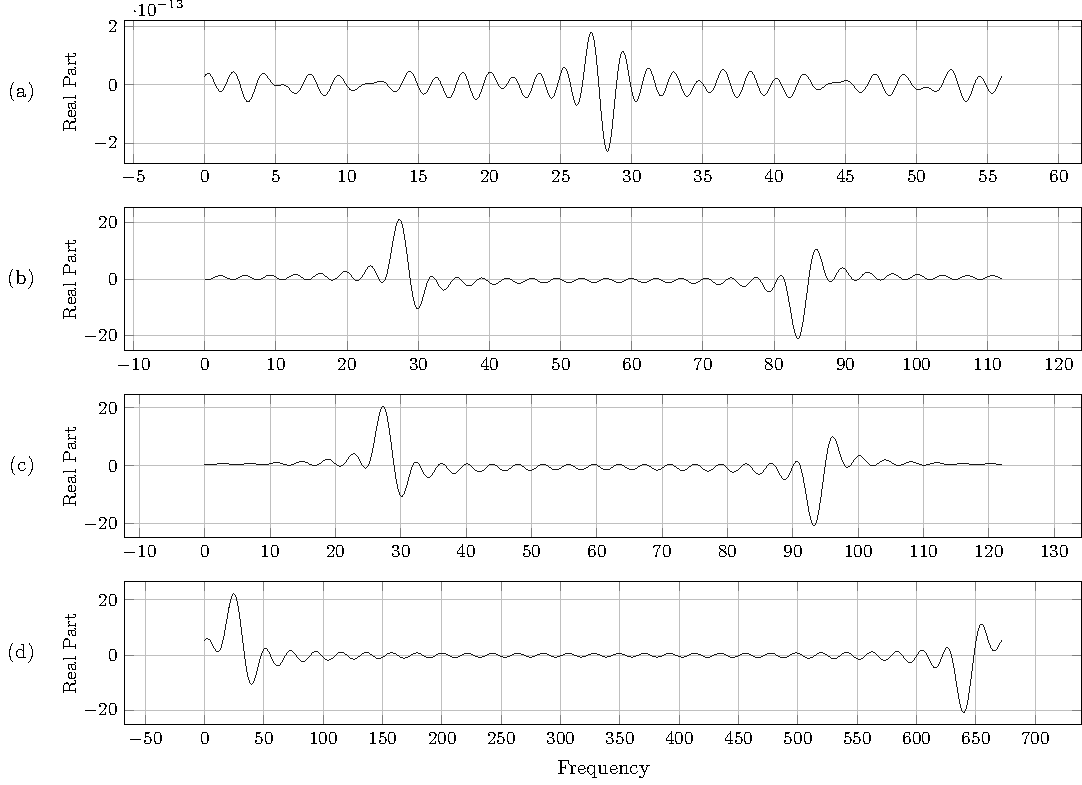
\includegraphics[height = 0.8\textheight] {tikzpics/plotDtftComplexA32.pdf}
    }
    \captionof{figure} {Plot of \textsc{dtft}s of \textsc{Complex A} with different sampling frequencies}
    \label{plt:dtftCplxA32}
\end{figure}

\subsubsection{DTFT with 64 Samples}

\begin{itemize} [label=]

    \item \sampFreqMuchLess
        \begin{itemize} [label=]
            \item
        \end{itemize}

    \item \sampFreqNorm
        \begin{itemize} [label=]
            \item
        \end{itemize}

    \item \sampFreqSligGreat
        \begin{itemize} [label=]
            \item
        \end{itemize}

    \item \sampFreqMuchGreat
        \begin{itemize} [label=]
            \item
        \end{itemize}

    \item \textbf{Inference:} Looks like this is similar to $32$ samples. The padding of $32$
        zero didn't make any difference.

\end{itemize}


\vfill

\begin{figure} [H]
    \centering
    \adjustbox{max width = 1\textwidth} {
        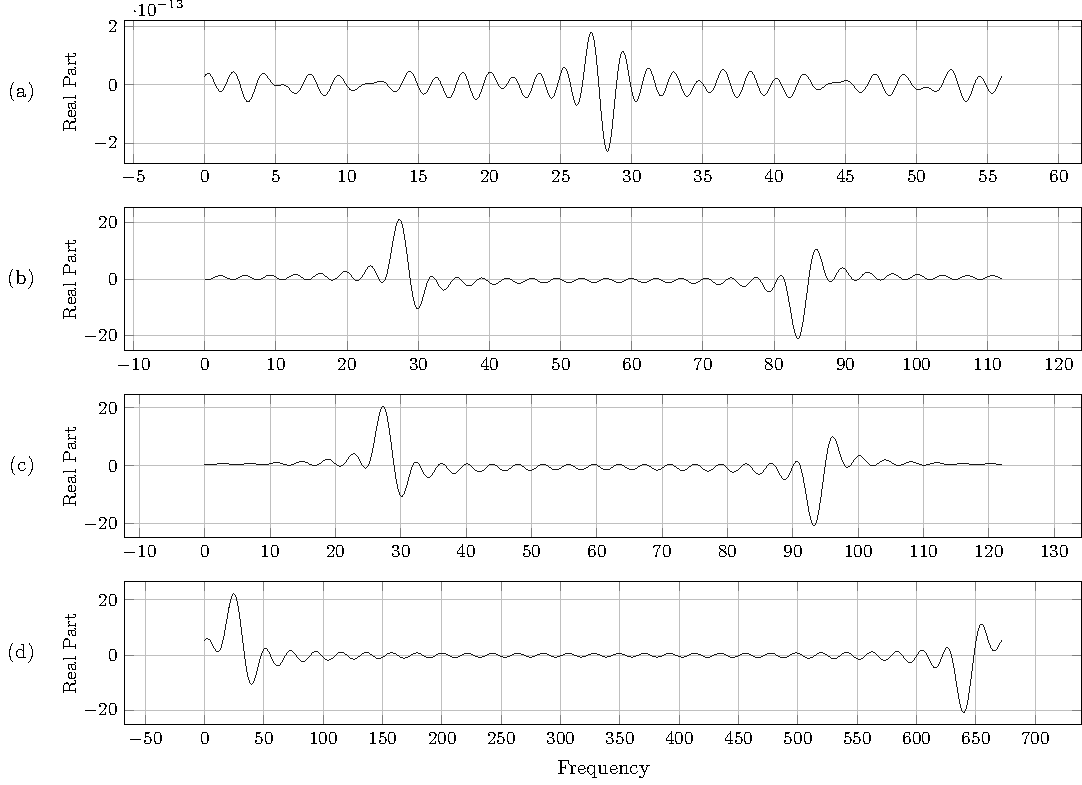
\includegraphics[height = 0.8\textheight] {tikzpics/plotDtftComplexA64.pdf}
    }
    \captionof{figure} {Plot of \textsc{dtft}s of \textsc{Complex A} with different sampling frequencies}
    \label{plt:dtftCplxA64}
\end{figure}

\pagebreak

\subsection{DTFT of Complex B} \label{ssec:dtftCplxB}

\begin{itemize} [label=]

    \item \textbf{Sequence:} $\sin(2 \pi \freqXOne t) + j \sin(2 \pi \freqXTwo t)$

\end{itemize}

\subsubsection{DTFT with 32 Samples}

\begin{itemize} [label=]

    \item \sampFreqMuchLess
        \begin{itemize} [label=]
            \item To much \emph{aliasing}, nothing can be inferred.
        \end{itemize}

    \item \sampFreqNorm
        \begin{itemize} [label=]
            \item We can see $\freqXOne \si{Hz}$ but no sign of $\freqXTwo \si{Hz}$
        \end{itemize}

    \item \sampFreqSligGreat
        \begin{itemize} [label=]
            \item We can see both the frequencies. \emph{Real} frequency $\freqXOne \si{Hz}$
                is at the \emph{zero crossing} of the first impulse, and the \emph{imaginary}
                frequency $\freqXTwo \si{Hz}$ is at the \emph{tip} of the second pulse.
        \end{itemize}

    \item \sampFreqMuchGreat
        \begin{itemize} [label=]
            \item Similar to (c), but a bit hard to distinguish.
        \end{itemize}

    \item \textbf{Inference:} It's looks like the frequency of \emph{sine} in the \emph{real}
        part can be found as a \emph{zero crossing} \emph{N} shaped pulse. And a frequency of \emph{sine}
        in \emph{imaginary} part can be found at the \emph{tip} of an \emph{impulse} shaped pulse.


\end{itemize}

\vfill

\begin{figure} [H]
    \centering
    \adjustbox{max width = 1\textwidth} {
        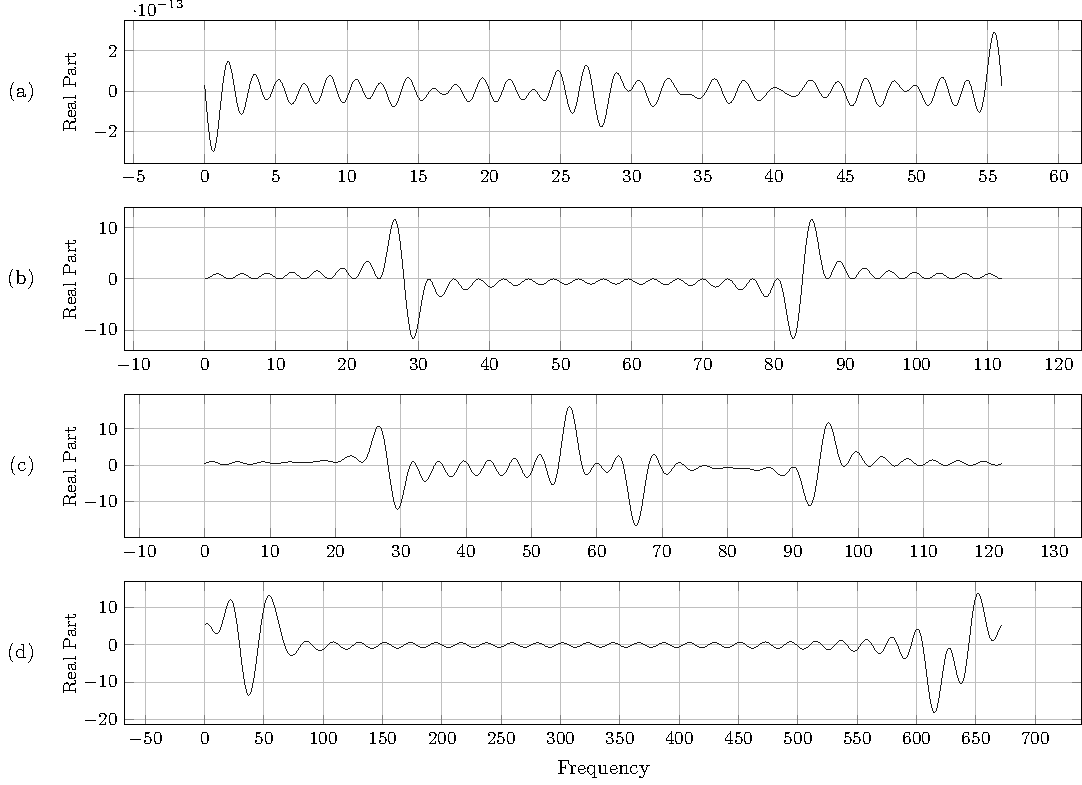
\includegraphics[height = 0.8\textheight] {tikzpics/plotDtftComplexB32.pdf}
    }
    \captionof{figure} {Plot of \textsc{dtft}s of \textsc{Complex B} with different sampling frequencies}
    \label{plt:dtftCplxB32}
\end{figure}

\subsubsection{DTFT with 64 Samples}

\begin{itemize} [label=]

    \item \sampFreqMuchLess
        \begin{itemize} [label=]
            \item
        \end{itemize}

    \item \sampFreqNorm
        \begin{itemize} [label=]
            \item
        \end{itemize}

    \item \sampFreqSligGreat
        \begin{itemize} [label=]
            \item
        \end{itemize}

    \item \sampFreqMuchGreat
        \begin{itemize} [label=]
            \item
        \end{itemize}

    \item \textbf{Inference:} Similar to $32$ point, padding made no difference.

\end{itemize}


\vfill

\begin{figure} [H]
    \centering
    \adjustbox{max width = 1\textwidth} {
        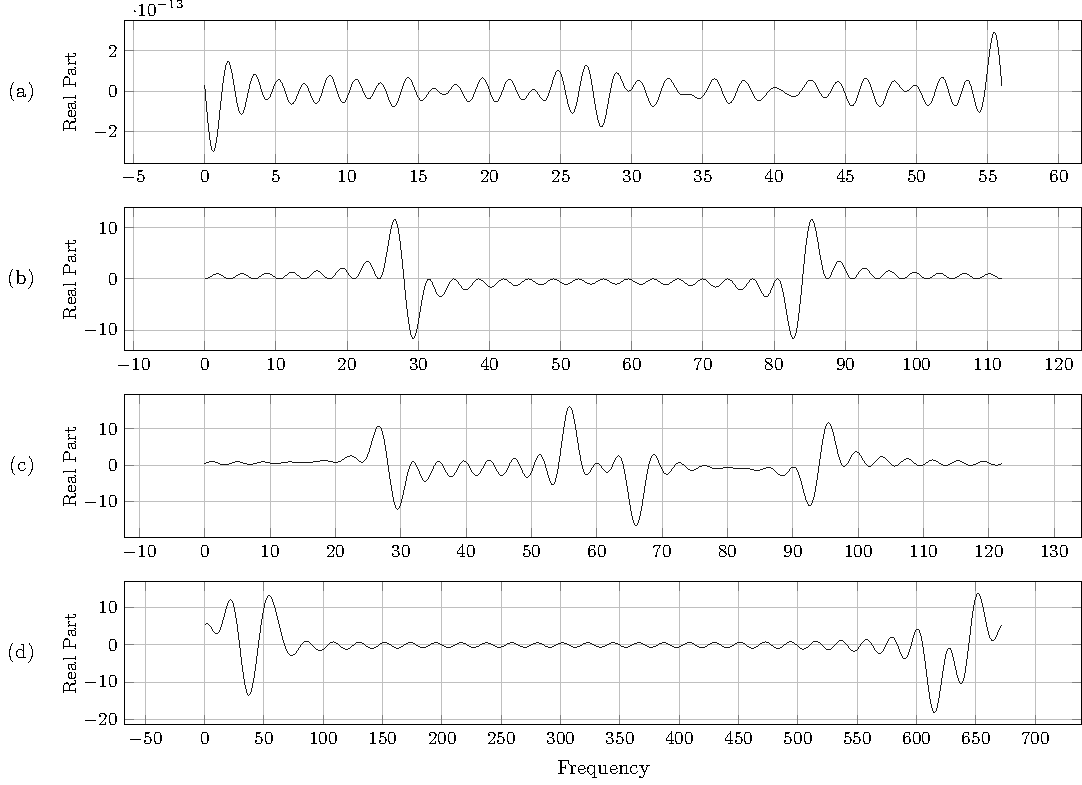
\includegraphics[height = 0.8\textheight] {tikzpics/plotDtftComplexB64.pdf}
    }
    \captionof{figure} {Plot of \textsc{dtft}s of \textsc{Complex B} with different sampling frequencies}
    \label{plt:dtftCplxB64}
\end{figure}

\pagebreak

\subsection{DTFT of Complex C} \label{ssec:dtftCplxC}

\begin{itemize} [label=]

    \item \textbf{Sequence:} $\sin(2 \pi \freqXOne t) + j \sin(2 \pi \freqXThree t)$

\end{itemize}

\subsubsection{DTFT with 32 Samples}

\begin{itemize} [label=]

    \item \sampFreqMuchLess
        \begin{itemize} [label=]
            \item Too much \emph{aliasing}.
        \end{itemize}

    \item \sampFreqNorm
        \begin{itemize} [label=]
            \item Only $\freqXOne \si{Hz}$ can be inferred.
        \end{itemize}

    \item \sampFreqSligGreat
        \begin{itemize} [label=]
            \item Both can be inferred, but maybe hard to pinpoint the exact frequency of \emph{imaginary}
                part as $\freqXThree \si{Hz}$
        \end{itemize}

    \item \sampFreqMuchGreat
        \begin{itemize} [label=]
            \item Both can be inferred, kind of...
        \end{itemize}

    \item \textbf{Inference:} Similar to \textsc{Complex B}.

\end{itemize}

\vfill

\begin{figure} [H]
    \centering
    \adjustbox{max width = 1\textwidth} {
        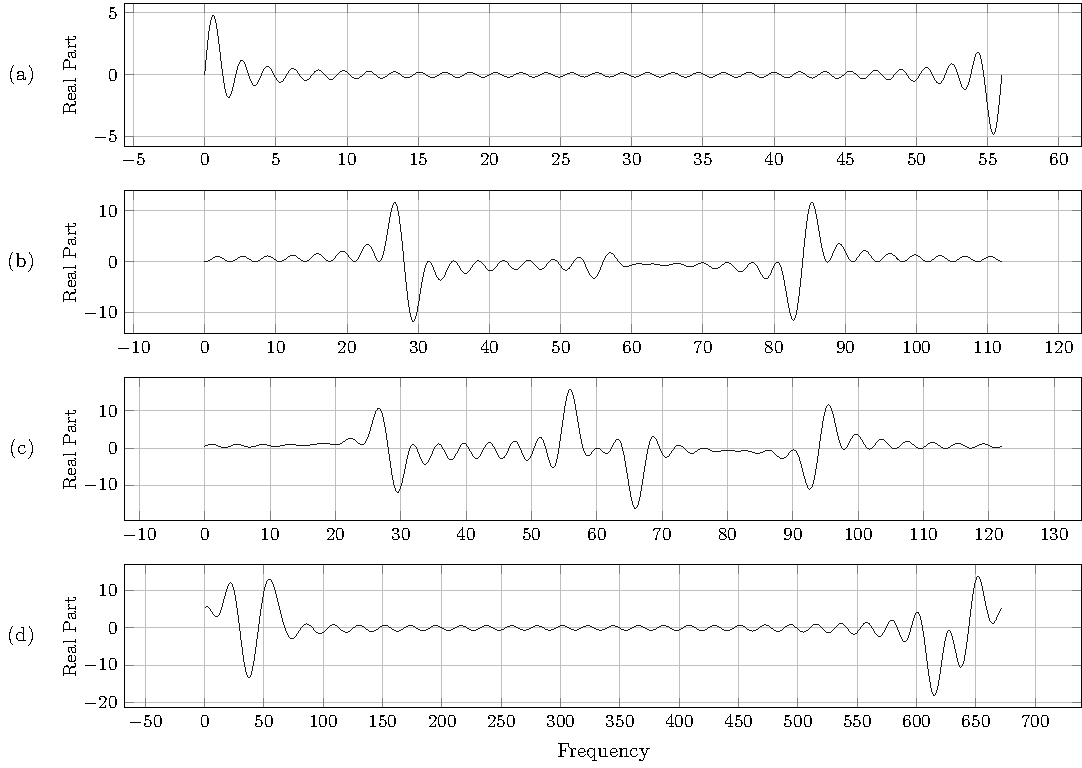
\includegraphics[height = 0.8\textheight] {tikzpics/plotDtftComplexC32.pdf}
    }
    \captionof{figure} {Plot of \textsc{dtft}s of \textsc{Complex C} with different sampling frequencies}
    \label{plt:dtftCplxC32}
\end{figure}

\subsubsection{DTFT with 64 Samples}

\begin{itemize} [label=]

    \item \sampFreqMuchLess
        \begin{itemize} [label=]
            \item
        \end{itemize}

    \item \sampFreqNorm
        \begin{itemize} [label=]
            \item
        \end{itemize}

    \item \sampFreqSligGreat
        \begin{itemize} [label=]
            \item
        \end{itemize}

    \item \sampFreqMuchGreat
        \begin{itemize} [label=]
            \item
        \end{itemize}

    \item \textbf{Inference:} Similar as $32$ point.

\end{itemize}


\vfill

\begin{figure} [H]
    \centering
    \adjustbox{max width = 1\textwidth} {
        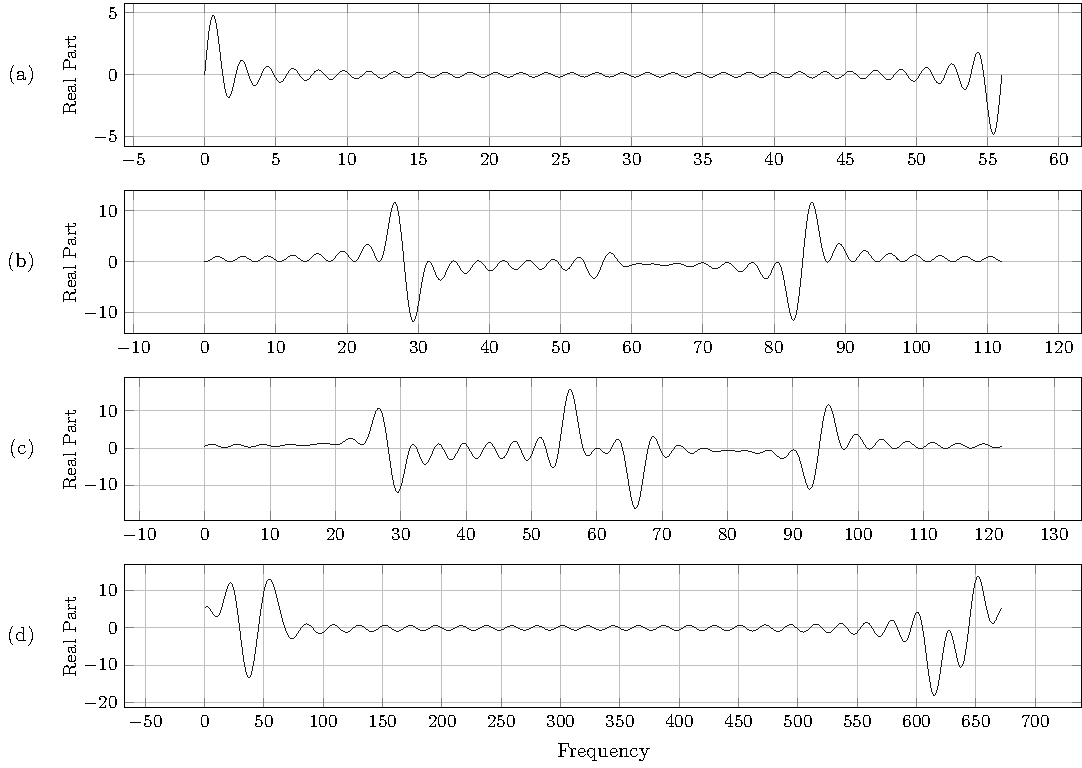
\includegraphics[height = 0.8\textheight] {tikzpics/plotDtftComplexC64.pdf}
    }
    \captionof{figure} {Plot of \textsc{dtft}s of \textsc{Complex C} with different sampling frequencies}
    \label{plt:dtftCplxC64}
\end{figure}

\pagebreak

\subsection{DTFT of Complex F} \label{ssec:dtftCplxF}

\begin{itemize} [label=]

    \item \textbf{Sequence:} $\sin(2 \pi \freqXTwo t) + j \sin(2 \pi \freqXThree t)$

\end{itemize}

\subsubsection{DTFT with 32 Samples}

\begin{itemize} [label=]

    \item \sampFreqMuchLess
        \begin{itemize} [label=]
            \item Too much \emph{aliasing}, causing to misidentify $1 \si{Hz}$ as one of the
                frequency components.
        \end{itemize}

    \item \sampFreqNorm
        \begin{itemize} [label=]
            \item Has \emph{aliasing}, barely identify $\freqXTwo \si{Hz}$.
        \end{itemize}

    \item \sampFreqSligGreat
        \begin{itemize} [label=]
            \item Can identify a bulging, but it would be hard to $\freqXThree \si{Hz}$ from $\freqXTwo \si{Hz}$.
        \end{itemize}

    \item \sampFreqMuchGreat
        \begin{itemize} [label=]
            \item Similar to (c).
        \end{itemize}

    \item \textbf{Inference:} Maybe we need much more \emph{samples} of the input sequence, to identify,
        closer \emph{frequencies}.

\end{itemize}

\vfill

\begin{figure} [H]
    \centering
    \adjustbox{max width = 1\textwidth} {
        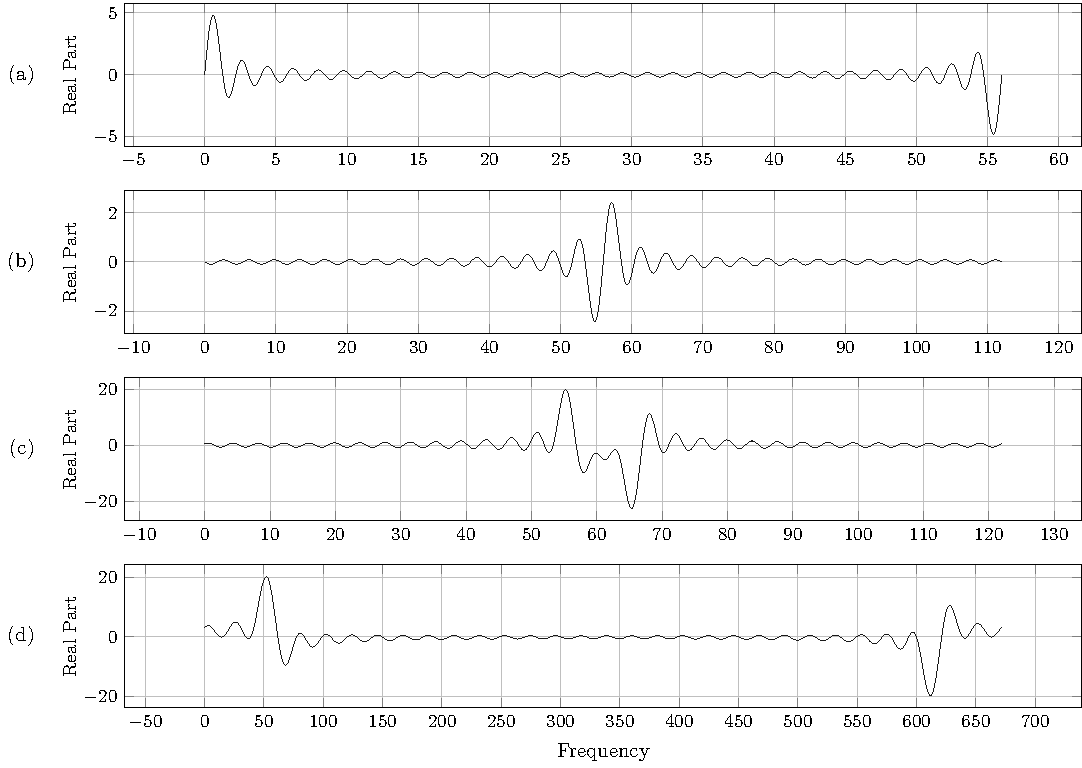
\includegraphics[height = 0.8\textheight] {tikzpics/plotDtftComplexF32.pdf}
    }
    \captionof{figure} {Plot of \textsc{dtft}s of \textsc{Complex F} with different sampling frequencies}
    \label{plt:dtftCplxF32}
\end{figure}

\subsubsection{DTFT with 64 Samples}

\begin{itemize} [label=]

    \item \sampFreqMuchLess
        \begin{itemize} [label=]
            \item
        \end{itemize}

    \item \sampFreqNorm
        \begin{itemize} [label=]
            \item
        \end{itemize}

    \item \sampFreqSligGreat
        \begin{itemize} [label=]
            \item
        \end{itemize}

    \item \sampFreqMuchGreat
        \begin{itemize} [label=]
            \item
        \end{itemize}

    \item \textbf{Inference:} Similar to $32$ point.

\end{itemize}


\vfill

\begin{figure} [H]
    \centering
    \adjustbox{max width = 1\textwidth} {
        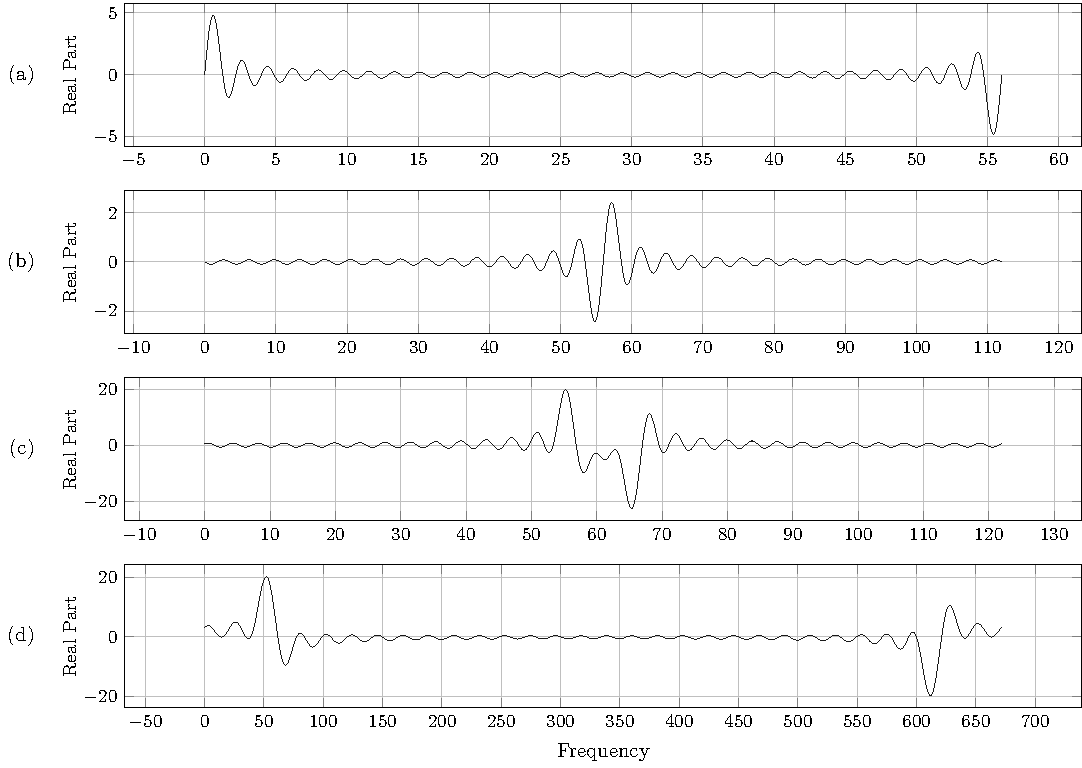
\includegraphics[height = 0.8\textheight] {tikzpics/plotDtftComplexF64.pdf}
    }
    \captionof{figure} {Plot of \textsc{dtft}s of \textsc{Complex F} with different sampling frequencies}
    \label{plt:dtftCplxF64}
\end{figure}

\pagebreak



%% In Sections \ref{sec:wrkGenSeqs} and \ref{sec:wrkGenCompSeqs}, we did

%%% A
%%% $x_{1} + j x_{1}$
%
%\textbf{Sequence:} $\sin(2 \pi \freqXOne t) + j \sin(2 \pi \freqXOne t)$
%
%%% B
%%% $x_{1} + j x_{2}$
%
%\textbf{Sequence:} $\sin(2 \pi \freqXOne t) + j \sin(2 \pi \freqXTwo t)$
%
%%% C
%%% $x_{1} + j x_{3}$
%
%\textbf{Sequence:} $\sin(2 \pi \freqXOne t) + j \sin(2 \pi \freqXThree t)$
%
%%% F
%%% $x_{2} + j x_{3}$
%\textbf{Sequence:} $\sin(2 \pi \freqXTwo t) + j \sin(2 \pi \freqXThree t)$
%
%%%  a, b, c, f


\end{document}
